\documentclass[11pt,fleqn, oneside,openany]{extbook} % Default font size and left-justified equations

% use this list: https://www.educative.io/blog/google-coding-interview

%%%%%%%%%%%%%%%%%%%%%%%%%%%%%%%%%%%%%%%%%%%%
%               Structure
%%%%%%%%%%%%%%%%%%%%%%%%%%%%%%%%%%%%%%%%%%%%
%%%%%%%%%%%%%%%%%%%%%%%%%%%%%%%%%%%%%%%%%
% The Legrand Orange Book
% Structural Definitions File
% Version 2.0 (9/2/15)
%
% Original author:
% Mathias Legrand (legrand.mathias@gmail.com) with modifications by:
% Vel (vel@latextemplates.com)
% 
% This file has been downloaded from:
% http://www.LaTeXTemplates.com
%
% License:
% CC BY-NC-SA 3.0 (http://creativecommons.org/licenses/by-nc-sa/3.0/)
%
%%%%%%%%%%%%%%%%%%%%%%%%%%%%%%%%%%%%%%%%%

%----------------------------------------------------------------------------------------
%	VARIOUS REQUIRED PACKAGES AND CONFIGURATIONS
%----------------------------------------------------------------------------------------

\usepackage[top=3cm,bottom=3cm,left=3cm,right=3cm,headsep=10pt,a4paper]{geometry} % Page margins

\usepackage{graphicx} % Required for including pictures
\graphicspath{{images/}} % Specifies the directory where pictures are stored

\usepackage{lipsum} % Inserts dummy text

\usepackage{tikz} % Required for drawing custom shapes

\usepackage[english]{babel} % English language/hyphenation

\usepackage{enumitem} % Customize lists
\setlist{nolistsep} % Reduce spacing between bullet points and numbered lists

\usepackage{booktabs} % Required for nicer horizontal rules in tables

\usepackage{xcolor} % Required for specifying colors by name
\definecolor{ocre}{RGB}{243,102,25} % Define the orange color used for highlighting throughout the book

%----------------------------------------------------------------------------------------
%	FONTS
%----------------------------------------------------------------------------------------

\usepackage{avant} % Use the Avantgarde font for headings
%\usepackage{times} % Use the Times font for headings
\usepackage{mathptmx} % Use the Adobe Times Roman as the default text font together with math symbols from the Sym­bol, Chancery and Com­puter Modern fonts

\usepackage{microtype} % Slightly tweak font spacing for aesthetics
\usepackage[utf8]{inputenc} % Required for including letters with accents
\usepackage[T1]{fontenc} % Use 8-bit encoding that has 256 glyphs

%----------------------------------------------------------------------------------------
%	BIBLIOGRAPHY AND INDEX
%----------------------------------------------------------------------------------------

\usepackage[citestyle=numeric,sorting=nyt,sortcites=true,autopunct=true,babel=hyphen,hyperref=true,abbreviate=false,backref=true,backend=biber]{biblatex}
\addbibresource{sources/bibliography.bib}
\defbibheading{bibempty}{}

\usepackage{calc} % For simpler calculation - used for spacing the index letter headings correctly
\usepackage{makeidx} % Required to make an index
\makeindex % Tells LaTeX to create the files required for indexing

%----------------------------------------------------------------------------------------
%	MAIN TABLE OF CONTENTS
%----------------------------------------------------------------------------------------

\usepackage{titletoc} % Required for manipulating the table of contents

\contentsmargin{0cm} % Removes the default margin

% Part text styling
\titlecontents{part}[0cm]
{\addvspace{20pt}\centering\large\bfseries}
{}
{}
{}

% Chapter text styling
\titlecontents{chapter}[1.25cm] % Indentation
{\addvspace{12pt}\large\sffamily\bfseries} % Spacing and font options for chapters
{\color{ocre!60}\contentslabel[\Large\thecontentslabel]{1.25cm}\color{ocre}} % Chapter number
{\color{ocre}}  
{\color{ocre!60}\normalsize\;\titlerule*[.5pc]{.}\;\thecontentspage} % Page number

% Section text styling
\titlecontents{section}[1.25cm] % Indentation
{\addvspace{3pt}\sffamily\bfseries} % Spacing and font options for sections
{\contentslabel[\thecontentslabel]{1.25cm}} % Section number
{}
{\hfill\color{black}\thecontentspage} % Page number
[]

% Subsection text styling
\titlecontents{subsection}[1.25cm] % Indentation
{\addvspace{1pt}\sffamily\small} % Spacing and font options for subsections
{\contentslabel[\thecontentslabel]{1.25cm}} % Subsection number
{}
{\ \titlerule*[.5pc]{.}\;\thecontentspage} % Page number
[]

% List of figures
\titlecontents{figure}[0em]
{\addvspace{-5pt}\sffamily}
{\thecontentslabel\hspace*{1em}}
{}
{\ \titlerule*[.5pc]{.}\;\thecontentspage}
[]

% List of tables
\titlecontents{table}[0em]
{\addvspace{-5pt}\sffamily}
{\thecontentslabel\hspace*{1em}}
{}
{\ \titlerule*[.5pc]{.}\;\thecontentspage}
[]

%----------------------------------------------------------------------------------------
%	MINI TABLE OF CONTENTS IN PART HEADS
%----------------------------------------------------------------------------------------

% Chapter text styling
\titlecontents{lchapter}[0em] % Indenting
{\addvspace{15pt}\large\sffamily\bfseries} % Spacing and font options for chapters
{\color{ocre}\contentslabel[\Large\thecontentslabel]{1.25cm}\color{ocre}} % Chapter number
{}  
{\color{ocre}\normalsize\sffamily\bfseries\;\titlerule*[.5pc]{.}\;\thecontentspage} % Page number

% Section text styling
\titlecontents{lsection}[0em] % Indenting
{\sffamily\small} % Spacing and font options for sections
{\contentslabel[\thecontentslabel]{1.25cm}} % Section number
{}
{}

% Subsection text styling
\titlecontents{lsubsection}[.5em] % Indentation
{\normalfont\footnotesize\sffamily} % Font settings
{}
{}
{}

%----------------------------------------------------------------------------------------
%	PAGE HEADERS
%----------------------------------------------------------------------------------------

\usepackage{fancyhdr} % Required for header and footer configuration

\pagestyle{fancy}
\renewcommand{\chaptermark}[1]{\markboth{\sffamily\normalsize\bfseries\chaptername\ \thechapter.\ #1}{}} % Chapter text font settings
\renewcommand{\sectionmark}[1]{\markright{\sffamily\normalsize\thesection\hspace{5pt}#1}{}} % Section text font settings
\fancyhf{} \fancyhead[LE,RO]{\sffamily\normalsize\thepage} % Font setting for the page number in the header
\fancyhead[LO]{\rightmark} % Print the nearest section name on the left side of odd pages
\fancyhead[RE]{\leftmark} % Print the current chapter name on the right side of even pages
\renewcommand{\headrulewidth}{0.5pt} % Width of the rule under the header
\addtolength{\headheight}{2.5pt} % Increase the spacing around the header slightly
\renewcommand{\footrulewidth}{0pt} % Removes the rule in the footer
\fancypagestyle{plain}{\fancyhead{}\renewcommand{\headrulewidth}{0pt}} % Style for when a plain pagestyle is specified

% Removes the header from odd empty pages at the end of chapters
\makeatletter
\renewcommand{\cleardoublepage}{
\clearpage\ifodd\c@page\else
\hbox{}
\vspace*{\fill}
\thispagestyle{empty}
\newpage
\fi}

%----------------------------------------------------------------------------------------
%	THEOREM STYLES
%----------------------------------------------------------------------------------------


\usepackage{amsmath,amsfonts,amssymb,amsthm,mathtools} % For math equations, theorems, symbols, etc
\DeclarePairedDelimiter\ceil{\lceil}{\rceil}
\DeclarePairedDelimiter\floor{\lfloor}{\rfloor}

\newcommand{\intoo}[2]{\mathopen{]}#1\,;#2\mathclose{[}}
\newcommand{\ud}{\mathop{\mathrm{{}d}}\mathopen{}}
\newcommand{\intff}[2]{\mathopen{[}#1\,;#2\mathclose{]}}
\newtheorem{notation}{Notation}[chapter]

% Boxed/framed environments
\newtheoremstyle{ocrenumbox}% % Theorem style name
{0pt}% Space above
{0pt}% Space below
{\normalfont}% % Body font
{}% Indent amount
{\small\bf\sffamily\color{ocre}}% % Theorem head font
{\;}% Punctuation after theorem head
{0.25em}% Space after theorem head
{\small\sffamily\color{ocre}\thmname{#1}\nobreakspace\thmnumber{\@ifnotempty{#1}{}\@upn{#2}}% Theorem text (e.g. Theorem 2.1)
\thmnote{\nobreakspace\the\thm@notefont\sffamily\bfseries\color{black}---\nobreakspace#3.}} % Optional theorem note
\renewcommand{\qedsymbol}{$\blacksquare$}% Optional qed square

\newtheoremstyle{blacknumex}% Theorem style name
{5pt}% Space above
{5pt}% Space below
{\normalfont}% Body font
{} % Indent amount
{\small\bf\sffamily}% Theorem head font
{\;}% Punctuation after theorem head
{0.25em}% Space after theorem head
{\small\sffamily{\tiny\ensuremath{\blacksquare}}\nobreakspace\thmname{#1}\nobreakspace\thmnumber{\@ifnotempty{#1}{}\@upn{#2}}% Theorem text (e.g. Theorem 2.1)
\thmnote{\nobreakspace\the\thm@notefont\sffamily\bfseries---\nobreakspace#3.}}% Optional theorem note

\newtheoremstyle{blacknumbox} % Theorem style name
{0pt}% Space above
{0pt}% Space below
{\normalfont}% Body font
{}% Indent amount
{\small\bf\sffamily}% Theorem head font
{\;}% Punctuation after theorem head
{0.25em}% Space after theorem head
{\small\sffamily\thmname{#1}\nobreakspace\thmnumber{\@ifnotempty{#1}{}\@upn{#2}}% Theorem text (e.g. Theorem 2.1)
\thmnote{\nobreakspace\the\thm@notefont\sffamily\bfseries---\nobreakspace#3.}}% Optional theorem note

% Non-boxed/non-framed environments
\newtheoremstyle{ocrenum}% % Theorem style name
{5pt}% Space above
{5pt}% Space below
{\normalfont}% % Body font
{}% Indent amount
{\small\bf\sffamily\color{ocre}}% % Theorem head font
{\;}% Punctuation after theorem head
{0.25em}% Space after theorem head
{\small\sffamily\color{ocre}\thmname{#1}\nobreakspace\thmnumber{\@ifnotempty{#1}{}\@upn{#2}}% Theorem text (e.g. Theorem 2.1)
\thmnote{\nobreakspace\the\thm@notefont\sffamily\bfseries\color{black}---\nobreakspace#3.}} % Optional theorem note
\renewcommand{\qedsymbol}{$\blacksquare$}% Optional qed square
\makeatother

% Defines the theorem text style for each type of theorem to one of the three styles above
\newcounter{dummy} 
\numberwithin{dummy}{section}
\theoremstyle{ocrenumbox}
\newtheorem{theoremeT}[dummy]{Theorem}

\newtheorem{problem}{Exercise}[chapter]
\newtheorem{exerciseT}{Problem}
\theoremstyle{blacknumex}
\newtheorem{solution}{Solution}[chapter]
\newtheorem{solutionT}{solution}[chapter]
\theoremstyle{blacknumex}
\newtheorem{exampleT}{Example}[chapter]
\theoremstyle{blacknumbox}
\newtheorem{vocabulary}{Vocabulary}[chapter]
\newtheorem{definitionT}{Definition}[section]
\newtheorem{corollaryT}[dummy]{Corollary}
\theoremstyle{ocrenum}
\newtheorem{proposition}[dummy]{Proposition}

%----------------------------------------------------------------------------------------
%	DEFINITION OF COLORED BOXES
%----------------------------------------------------------------------------------------

\RequirePackage[framemethod=default]{mdframed} % Required for creating the theorem, definition, exercise and corollary boxes

% Theorem box
\newmdenv[skipabove=7pt,
skipbelow=7pt,
backgroundcolor=black!5,
linecolor=ocre,
innerleftmargin=5pt,
innerrightmargin=5pt,
innertopmargin=5pt,
leftmargin=0cm,
rightmargin=0cm,
innerbottommargin=5pt]{tBox}

% Exercise box	  
\newmdenv[skipabove=7pt,
skipbelow=7pt,
rightline=false,
leftline=true,
topline=false,
bottomline=false,
backgroundcolor=ocre!10,
linecolor=ocre,
innerleftmargin=5pt,
innerrightmargin=5pt,
innertopmargin=5pt,
innerbottommargin=5pt,
leftmargin=0cm,
rightmargin=0cm,
linewidth=4pt]{eBox}	

% Definition box
\newmdenv[skipabove=7pt,
skipbelow=7pt,
rightline=false,
leftline=true,
topline=false,
bottomline=false,
linecolor=ocre,
innerleftmargin=5pt,
innerrightmargin=5pt,
innertopmargin=0pt,
leftmargin=0cm,
rightmargin=0cm,
linewidth=4pt,
innerbottommargin=0pt]{dBox}	

% Corollary box
\newmdenv[skipabove=7pt,
skipbelow=7pt,
rightline=false,
leftline=true,
topline=false,
bottomline=false,
linecolor=gray,
backgroundcolor=black!5,
innerleftmargin=5pt,
innerrightmargin=5pt,
innertopmargin=5pt,
leftmargin=0cm,
rightmargin=0cm,
linewidth=4pt,
innerbottommargin=5pt]{cBox}

% Creates an environment for each type of theorem and assigns it a theorem text style from the "Theorem Styles" section above and a colored box from above
\newenvironment{theorem}{\begin{tBox}\begin{theoremeT}}{\end{theoremeT}\end{tBox}}
\newenvironment{exercise}{\begin{eBox}\begin{exerciseT}}{\hfill{\color{ocre}\tiny\ensuremath{\blacksquare}}\end{exerciseT}\end{eBox}}				  
\newenvironment{definition}{\begin{dBox}\begin{definitionT}}{\end{definitionT}\end{dBox}}	
\newenvironment{example}{\begin{exampleT}}{\hfill{\tiny\ensuremath{\blacksquare}}\end{exampleT}}		
\newenvironment{corollary}{\begin{cBox}\begin{corollaryT}}{\end{corollaryT}\end{cBox}}	

%----------------------------------------------------------------------------------------
%	REMARK ENVIRONMENT
%----------------------------------------------------------------------------------------

\newenvironment{remark}{\par\vspace{10pt}\small % Vertical white space above the remark and smaller font size
\begin{list}{}{
\leftmargin=35pt % Indentation on the left
\rightmargin=25pt}\item\ignorespaces % Indentation on the right
\makebox[-2.5pt]{\begin{tikzpicture}[overlay]
\node[draw=ocre!60,line width=1pt,circle,fill=ocre!25,font=\sffamily\bfseries,inner sep=2pt,outer sep=0pt] at (-15pt,0pt){\textcolor{ocre}{R}};\end{tikzpicture}} % Orange R in a circle
\advance\baselineskip -1pt}{\end{list}\vskip5pt} % Tighter line spacing and white space after remark

%----------------------------------------------------------------------------------------
%	SECTION NUMBERING IN THE MARGIN
%----------------------------------------------------------------------------------------

\makeatletter
\renewcommand{\@seccntformat}[1]{\llap{\textcolor{ocre}{\csname the#1\endcsname}\hspace{1em}}}                    
\renewcommand{\section}{\@startsection{section}{1}{\z@}
{-4ex \@plus -1ex \@minus -.4ex}
{1ex \@plus.2ex }
{\normalfont\large\sffamily\bfseries}}
\renewcommand{\subsection}{\@startsection {subsection}{2}{\z@}
{-3ex \@plus -0.1ex \@minus -.4ex}
{0.5ex \@plus.2ex }
{\normalfont\sffamily\bfseries}}
\renewcommand{\subsubsection}{\@startsection {subsubsection}{3}{\z@}
{-2ex \@plus -0.1ex \@minus -.2ex}
{.2ex \@plus.2ex }
{\normalfont\small\sffamily\bfseries}}                        
\renewcommand\paragraph{\@startsection{paragraph}{4}{\z@}
{-2ex \@plus-.2ex \@minus .2ex}
{.1ex}
{\normalfont\small\sffamily\bfseries}}

%----------------------------------------------------------------------------------------
%	PART HEADINGS
%----------------------------------------------------------------------------------------

% numbered part in the table of contents
\newcommand{\@mypartnumtocformat}[2]{%
\setlength\fboxsep{0pt}%
\noindent\colorbox{ocre!20}{\strut\parbox[c][.7cm]{\ecart}{\color{ocre!70}\Large\sffamily\bfseries\centering#1}}\hskip\esp\colorbox{ocre!40}{\strut\parbox[c][.7cm]{\linewidth-\ecart-\esp}{\Large\sffamily\centering#2}}}%
%%%%%%%%%%%%%%%%%%%%%%%%%%%%%%%%%%
% unnumbered part in the table of contents
\newcommand{\@myparttocformat}[1]{%
\setlength\fboxsep{0pt}%
\noindent\colorbox{ocre!40}{\strut\parbox[c][.7cm]{\linewidth}{\Large\sffamily\centering#1}}}%
%%%%%%%%%%%%%%%%%%%%%%%%%%%%%%%%%%
\newlength\esp
\setlength\esp{4pt}
\newlength\ecart
\setlength\ecart{1.2cm-\esp}
\newcommand{\thepartimage}{}%
\newcommand{\partimage}[1]{\renewcommand{\thepartimage}{#1}}%
\def\@part[#1]#2{%
\ifnum \c@secnumdepth >-2\relax%
\refstepcounter{part}%
\addcontentsline{toc}{part}{\texorpdfstring{\protect\@mypartnumtocformat{\thepart}{#1}}{\partname~\thepart\ ---\ #1}}
\else%
\addcontentsline{toc}{part}{\texorpdfstring{\protect\@myparttocformat{#1}}{#1}}%
\fi%
\startcontents%
\markboth{}{}%
{\thispagestyle{empty}%
\begin{tikzpicture}[remember picture,overlay]%
\node at (current page.north west){\begin{tikzpicture}[remember picture,overlay]%	
\fill[ocre!20](0cm,0cm) rectangle (\paperwidth,-\paperheight);
\node[anchor=north] at (4cm,-3.25cm){\color{ocre!40}\fontsize{220}{100}\sffamily\bfseries\@Roman\c@part}; 
\node[anchor=south east] at (\paperwidth-1cm,-\paperheight+1cm){\parbox[t][][t]{8.5cm}{
\printcontents{l}{0}{\setcounter{tocdepth}{1}}%
}};
\node[anchor=north east] at (\paperwidth-1.5cm,-3.25cm){\parbox[t][][t]{15cm}{\strut\raggedleft\color{white}\fontsize{30}{30}\sffamily\bfseries#2}};
\end{tikzpicture}};
\end{tikzpicture}}%
\@endpart}
\def\@spart#1{%
\startcontents%
\phantomsection
{\thispagestyle{empty}%
\begin{tikzpicture}[remember picture,overlay]%
\node at (current page.north west){\begin{tikzpicture}[remember picture,overlay]%	
\fill[ocre!20](0cm,0cm) rectangle (\paperwidth,-\paperheight);
\node[anchor=north east] at (\paperwidth-1.5cm,-3.25cm){\parbox[t][][t]{15cm}{\strut\raggedleft\color{white}\fontsize{30}{30}\sffamily\bfseries#1}};
\end{tikzpicture}};
\end{tikzpicture}}
\addcontentsline{toc}{part}{\texorpdfstring{%
\setlength\fboxsep{0pt}%
\noindent\protect\colorbox{ocre!40}{\strut\protect\parbox[c][.7cm]{\linewidth}{\Large\sffamily\protect\centering #1\quad\mbox{}}}}{#1}}%
\@endpart}
\def\@endpart{\vfil\newpage
\if@twoside
\if@openright
\null
\thispagestyle{empty}%
\newpage
\fi
\fi
\if@tempswa
\twocolumn
\fi}

%----------------------------------------------------------------------------------------
%	CHAPTER HEADINGS
%----------------------------------------------------------------------------------------

% A switch to conditionally include a picture, implemented by  Christian Hupfer
\newif\ifusechapterimage
\usechapterimagetrue
\newcommand{\thechapterimage}{}%
\newcommand{\chapterimage}[1]{\ifusechapterimage\renewcommand{\thechapterimage}{#1}\fi}%
\def\@makechapterhead#1{%
{\parindent \z@ \raggedright \normalfont
\ifnum \c@secnumdepth >\m@ne
\if@mainmatter
\begin{tikzpicture}[remember picture,overlay]
\node at (current page.north west)
{\begin{tikzpicture}[remember picture,overlay]
\node[anchor=north west,inner sep=0pt] at (0,0) {\ifusechapterimage\includegraphics[width=\paperwidth]{\thechapterimage}\fi};
\draw[anchor=west] (\Gm@lmargin,-4cm) node [line width=2pt,rounded corners=15pt,draw=ocre,fill=white,fill opacity=0.5,inner sep=15pt]{\strut\makebox[22cm]{}};
\draw[anchor=west] (\Gm@lmargin+.3cm,-4cm) node {\huge\sffamily\bfseries\color{black}\thechapter. #1\strut};
\end{tikzpicture}};
\end{tikzpicture}
\else
\begin{tikzpicture}[remember picture,overlay]
\node at (current page.north west)
{\begin{tikzpicture}[remember picture,overlay]
\node[anchor=north west,inner sep=0pt] at (0,0) {\ifusechapterimage\includegraphics[width=\paperwidth]{\thechapterimage}\fi};
\draw[anchor=west] (\Gm@lmargin,-4cm) node [line width=2pt,rounded corners=15pt,draw=ocre,fill=white,fill opacity=0.5,inner sep=15pt]{\strut\makebox[22cm]{}};
\draw[anchor=west] (\Gm@lmargin+.3cm,-4cm) node {\huge\sffamily\bfseries\color{black}#1\strut};
\end{tikzpicture}};
\end{tikzpicture}
\fi\fi\par\vspace*{100\p@}}}

%-------------------------------------------

\def\@makeschapterhead#1{%
\begin{tikzpicture}[remember picture,overlay]
\node at (current page.north west)
{\begin{tikzpicture}[remember picture,overlay]
\node[anchor=north west,inner sep=0pt] at (0,0) {\ifusechapterimage\includegraphics[width=\paperwidth]{\thechapterimage}\fi};
\draw[anchor=west] (\Gm@lmargin,-4cm) node [line width=2pt,rounded corners=15pt,draw=ocre,fill=white,fill opacity=0.5,inner sep=15pt]{\strut\makebox[22cm]{}};
\draw[anchor=west] (\Gm@lmargin+.3cm,-4cm) node {\huge\sffamily\bfseries\color{black}#1\strut};
\end{tikzpicture}};
\end{tikzpicture}
\par\vspace*{100\p@}}
\makeatother

%----------------------------------------------------------------------------------------
%	HYPERLINKS IN THE DOCUMENTS
%----------------------------------------------------------------------------------------

\usepackage{hyperref}
\hypersetup{hidelinks,backref=true,pagebackref=true,hyperindex=true,colorlinks=false,breaklinks=true,urlcolor= ocre,bookmarks=true,bookmarksopen=false,pdftitle={Title},pdfauthor={Author}}
\usepackage{bookmark}
\bookmarksetup{
open,
numbered,
addtohook={%
\ifnum\bookmarkget{level}=0 % chapter
\bookmarksetup{bold}%
\fi
\ifnum\bookmarkget{level}=-1 % part
\bookmarksetup{color=ocre,bold}%
\fi
}
}

%----------------------------------------------------------------------------------------
%	LISTINGS
%----------------------------------------------------------------------------------------
%----------------------------------------------------------------------------------------
%	LISTINGS
%----------------------------------------------------------------------------------------
\usepackage{listings}
\lstset{language=C++}
\lstset{
	basicstyle=\footnotesize\ttfamily,
	breaklines=true,
	showstringspaces=false,
	numbers=left,
	backgroundcolor=\color{bgcolor},
	commentstyle=\color{gray},
	keywordstyle=\color{blue},
	keywordstyle=[2]\color{teal},   % cyan or teal can also be a good choice, use \bfseries for bold
	frame=none,                     % adds a frame around the code
	tabsize=2,                      % sets default tabsize to 2 spaces
	captionpos=b,                   % sets the caption-position to bottom
	morekeywords=[2]{}              % if you want to add more keywords to the set
	__
}

\definecolor{mygreen}{RGB}{28,172,0} % color values Red, Green, Blue
\definecolor{mylilas}{RGB}{170,55,241}
\lstset{language=Matlab,%
    %basicstyle=\color{red},
    breaklines=true,%
    morekeywords={matlab2tikz},
    keywordstyle=\color{blue},%
    morekeywords=[2]{1}, keywordstyle=[2]{\color{black}},
    identifierstyle=\color{black},%
    stringstyle=\color{mylilas},
    commentstyle=\color{mygreen},%
    showstringspaces=false,%without this there will be a symbol in the places where there is a space
    numbers=left,%
    numberstyle={\tiny \color{black}},% size of the numbers
    numbersep=9pt, % this defines how far the numbers are from the text
    emph=[1]{for,end,break},emphstyle=[1]\color{red}, %some words to emphasise
    %emph=[2]{word1,word2}, emphstyle=[2]{style},    
}

\usepackage{color}
\definecolor{bgcolor}{rgb}{0.98,0.98,0.98}


%----------------------------------------------------------------------------------------

%	QandA

%----------------------------------------------------------------------------------------

\newenvironment{QandA}{\begin{enumerate}[label=\bfseries Q.\arabic*.,leftmargin=2em,rightmargin=2em]\bfseries}{\end{enumerate}}
\newenvironment{answered}{\par\normalfont}{}
%----------------------------------------------------------------------------------------
%	ALGORITHM
%----------------------------------------------------------------------------------------
\usepackage[]{algorithm2e}

\RestyleAlgo{boxruled}
\usepackage{mdframed,framed}

\SetKwProg{Fn}{Function}{}{}
\SetKwRepeat{Do}{do}{while}%
\SetKwFunction{CreateHashSet}{CreateHashSet<int>}


\DeclarePairedDelimiter\abs{\lvert}{\rvert}%
\DeclarePairedDelimiter\norm{\lVert}{\rVert}%

% Swap the definition of \abs* and \norm*, so that \abs
% and \norm resizes the size of the brackets, and the 
% starred version does not.
\makeatletter
\let\oldabs\abs
\def\abs{\@ifstar{\oldabs}{\oldabs*}}
%
\let\oldnorm\norm
\def\norm{\@ifstar{\oldnorm}{\oldnorm*}}
\makeatother

\usepackage[makeroom]{cancel}


\interfootnotelinepenalty=10000

\begin{document}

%\frontmatter
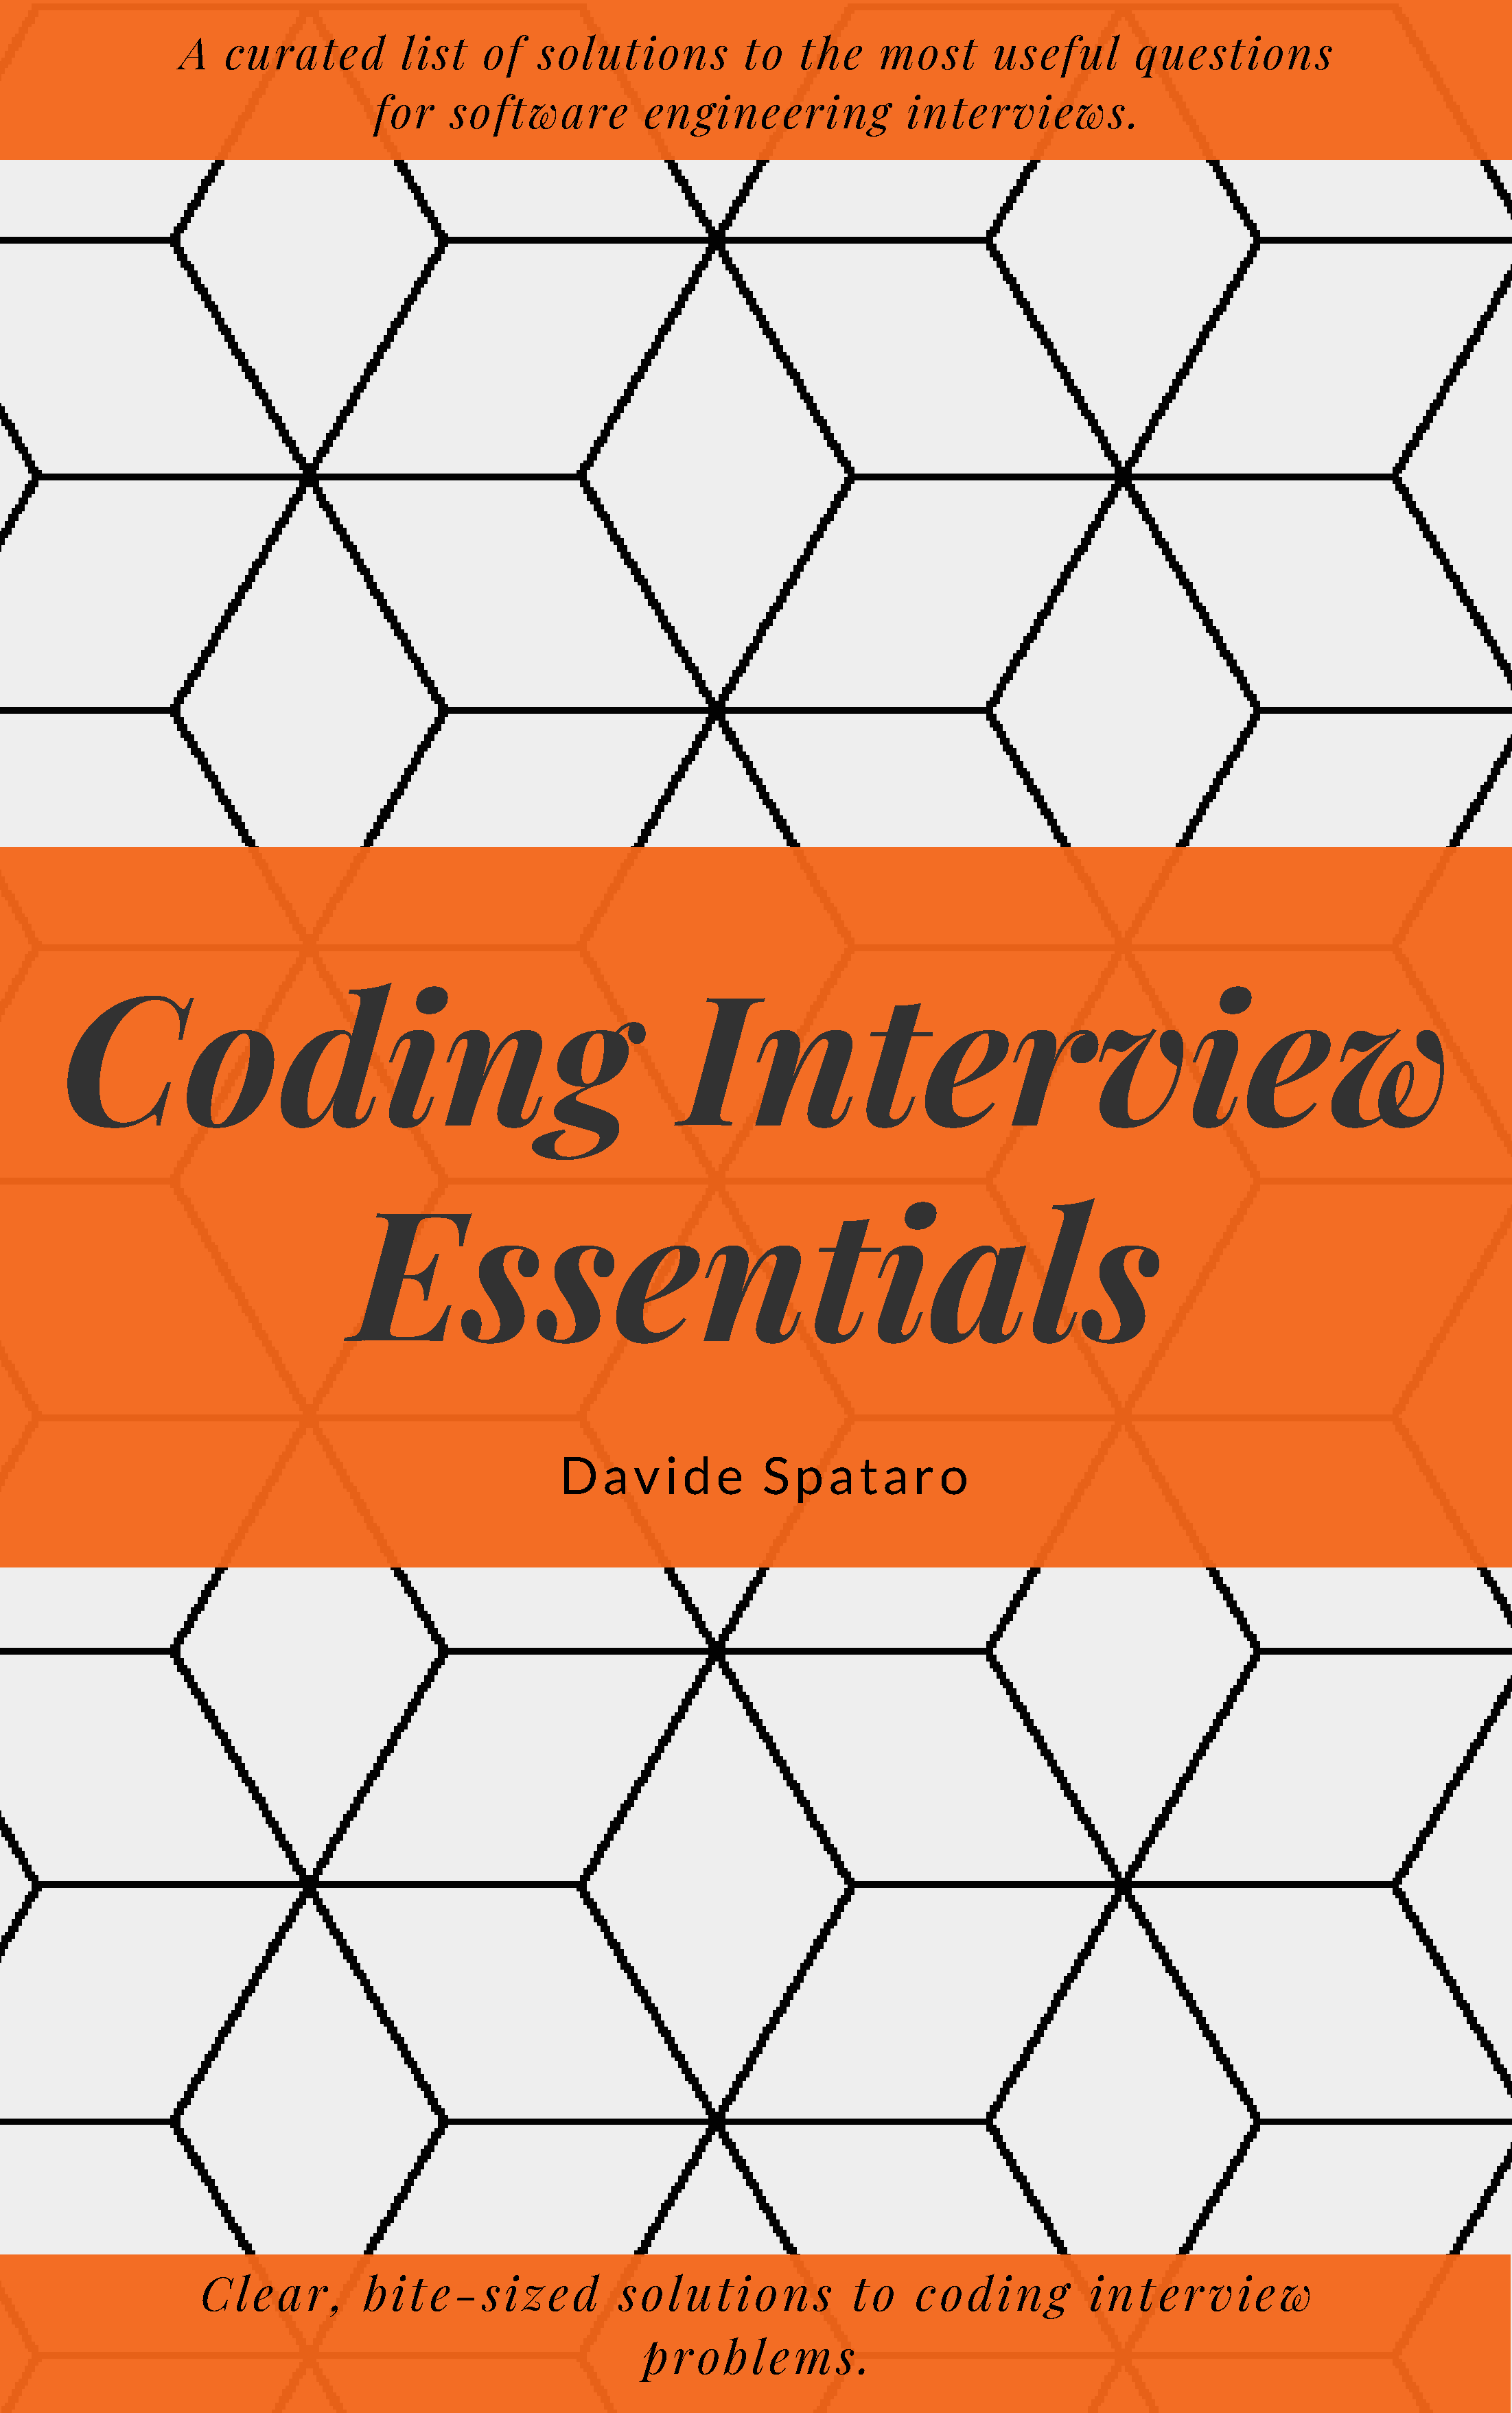
\includepdf[pages=1, fitpaper]{sources/front_cover_image.pdf}
%%\begingroup
%\thispagestyle{empty}
%\begin{tikzpicture}[remember picture,overlay]
%  \coordinate [below=12cm] (midpoint) at (current page.north);
%  \node at (current page.north west)
%  {\begin{tikzpicture}[remember picture,overlay]
%      \node[anchor=north west,inner sep=0pt] at (0,0) {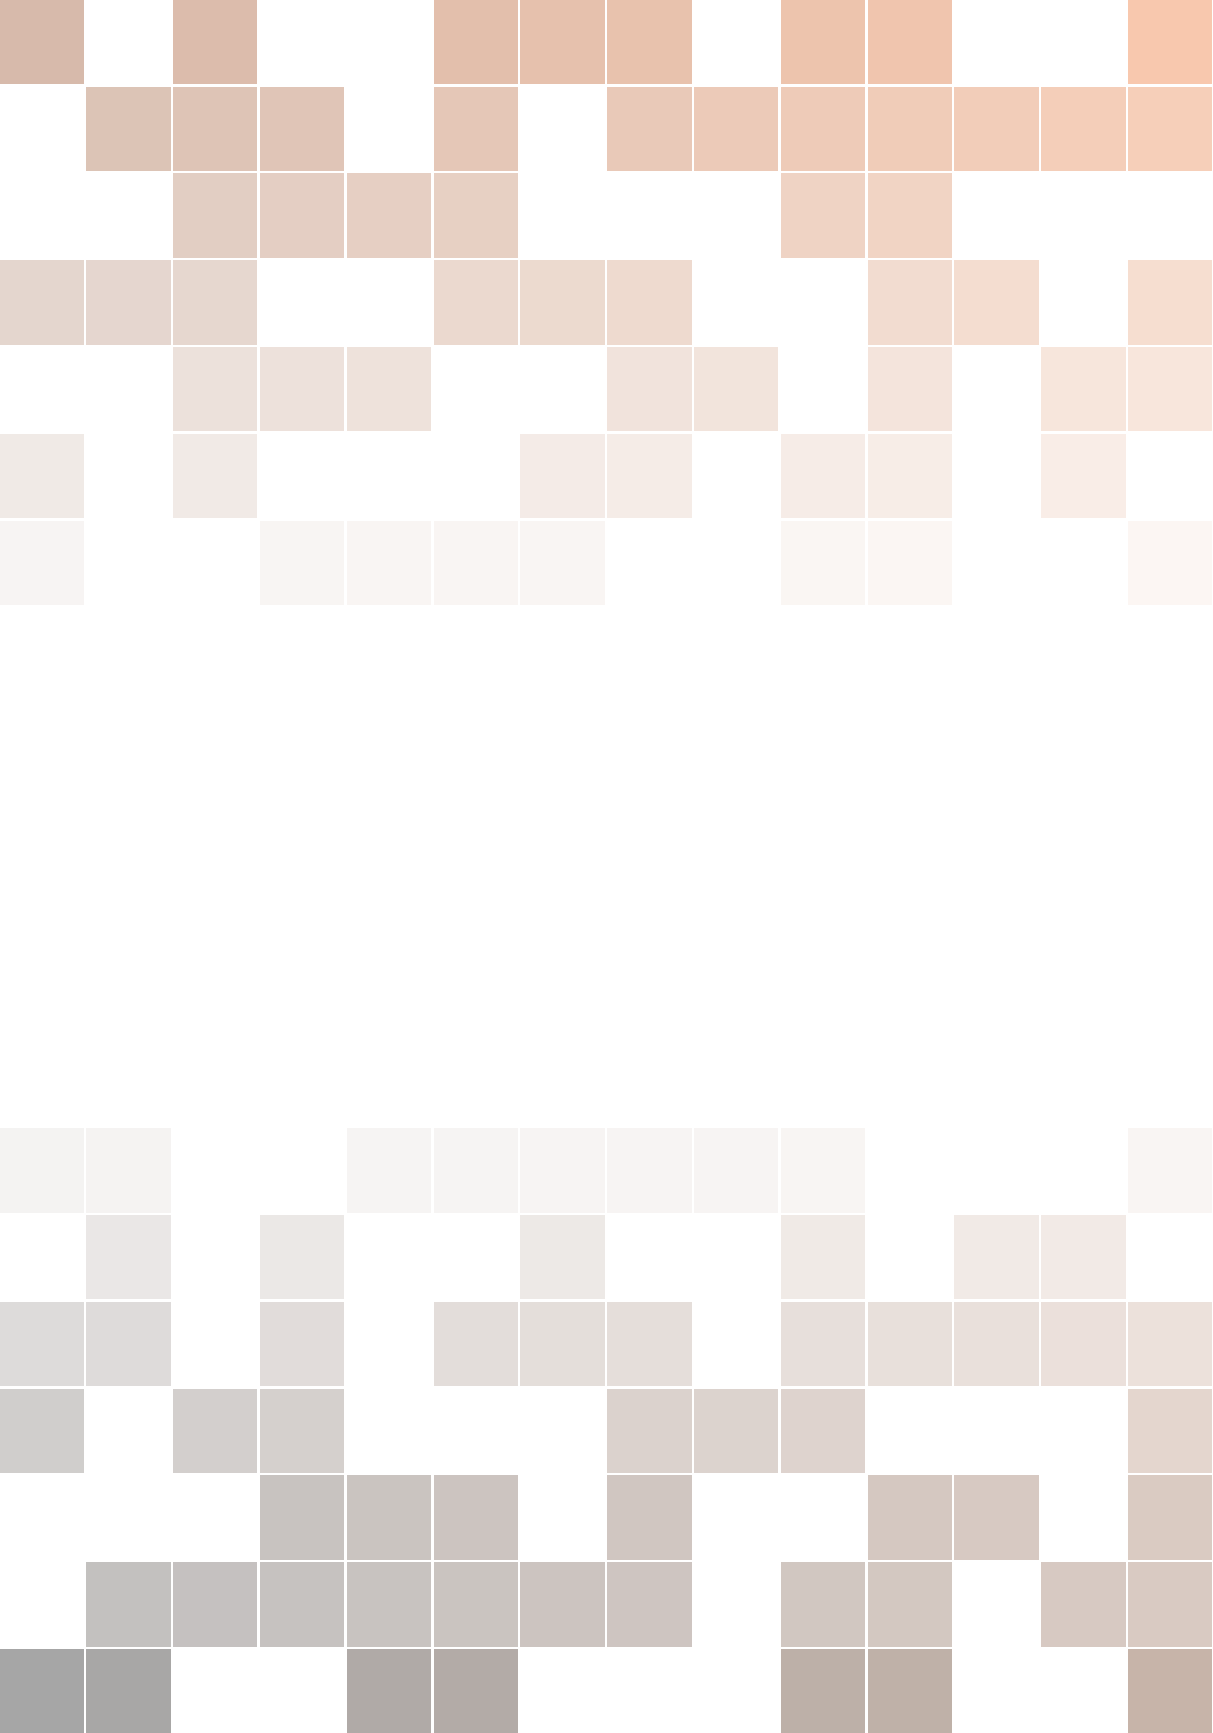
\includegraphics[width=\paperwidth]{images/background}}; % Background image
%\textsl{}
%      \draw[anchor=north] (midpoint) node [fill=ocre!30!white,fill opacity=0.6,text opacity=1,inner sep=1cm]{\Huge\centering\bfseries\sffamily\parbox[c][][t]{\paperwidth}{\centering Coding Interview Essentials\\[15pt] % Book title
%      {\Large - }\\[20pt] % Subtitle
%      {\huge Davide Spataro}}}; % Author name
%    \end{tikzpicture}};
%\end{tikzpicture}
%\vfill
%\endgroup


\includepdf[pages={2},fitpaper=true]{images/book_covers1.pdf}


\usechapterimagefalse % If you don't want to include a chapter image, use this to toggle images off - it can be enabled later with \usechapterimagetrue

%\chapterimage{images/header} % Table of contents heading image

\pagestyle{empty} % No headers

\tableofcontents % Print the table of contents itself

%\lstlistoflistings
%\listoffigures
%\listoftables

\cleardoublepage % Forces the first chapter to start on an odd page so it's on the right

%pagestyle{fancy} % Print headers again
%!TEX root = ../main.tex
%%%%%%%%%%%%%%%%%%%%%%%%%%%%%%%%%%
% Links:
%
% Difficulty:
% Companies: 
%%%%%%%%%%%%%%%%%%%%%%%%%%%%%%%%%%


%\begin{figure}
%   \centering
%   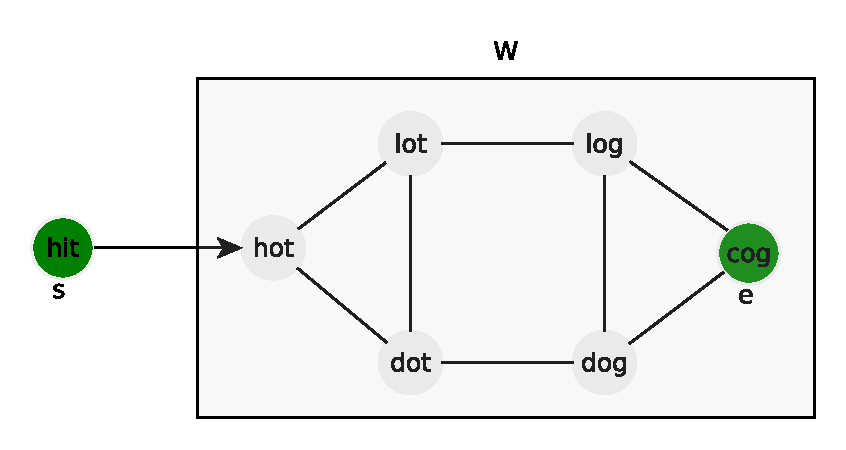
\includegraphics[width=\textwidth]{sources/word_ladder/images/example1}
%   \caption[Sample short cpation]{Sample Caption}.
%   \label{fig:word_ladder:example1}
%\end{figure}

\chapter{Word Ladder}
\label{ch:word_ladder}
\section*{Introduction}
\begin{wrapfigure}{r}{0.1\textwidth}
    \vspace{-30pt}
    \begin{center}
        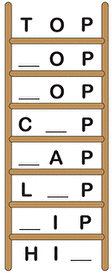
\includegraphics[scale=0.5]{sources/word_ladder/images/top-word-ladder}
    \end{center}
  \end{wrapfigure}
String is a popular topic in coding interviews and there are literally countless examples of real-world interviews where strings are involved in some way or another.
This manuscript already contains several string questions in chapters: \ref{ch:string_to_int} (page \pageref{ch:string_to_int}), \ref{ch:string_reverse} (page \pageref{ch:string_reverse}) and \ref{ch:two_string_anagram} (page \pageref{ch:two_string_anagram})).
Among this plethora of questions, \textit{word ladder} is definitely one of the most known and feared (at the time of writing it has one of the lowest acceptance rates on \href{https://leetcode.com/problems/word-ladder/}{leetcode.com}), as is considered a quite challenging and hard problem to solve during a live coding interview. 
We feel however that its bad reputation is unjustified because, as we will see below, it can be approached by using known algorithmic tools and concepts when framed as a graph connectivity problem.


\section{Problem statement}
\begin{exercise}
\label{example:word_ladder:exercice1}
We are given two strings $s$ and $e$ and a list of strings $W=\{w_0, w_1,\ldots,w_{n-1}\}$ of size $n$.
Let a sequence $S=s_0 = s \rightarrow s_1 \rightarrow s_2 \rightarrow \ldots \rightarrow s_n = e$ be defined as a \textit{transformation} if and only if:
\begin{itemize}
    \item $s_i$ differs from from its adjecent neighboring strings in the sequence, $s_{i-1}$ and $s_{i+1}$, in exactly one character;
    \item each elements of the sequence, from second to last, is also in $W$ i.e. $s_i \in W \: \: 1 \leq n-1 $
\end{itemize}
Write a function that given $s,e$ and $W$ returns the length of the smallest valid transformation.
If no transformation exists the function should return $0$.

    %example1
    \begin{example}
        \label{example:word_ladder:example1}
        \hfill \\
        Given $s=$\textit{hit},  $e=$\textit{cog} and $W=\{$\textit{hot},\textit{dot},\textit{dog},\textit{lot},\textit{log},\textit{cog}$\}$, the function returns $5$.
        A possible valid transformation  of minimal length is: \textit{hit} $\rightarrow$ \textit{hot} $\rightarrow$ \textit{dot} $\rightarrow$ \textit{dog} $\rightarrow$ \textit{cog}.

        Notice that if for instance $e=$\textit{fog}, the the function would return $0$ as \textit{fog} $\notin W$.
    \end{example}

\end{exercise}

\section{Clarification Questions}

\begin{QandA}
    \item What is the maximum length of each word in $W$?
    \begin{answered}
        \textit{Up to $10$ characters.}
    \end{answered}
    
    \item Is it guaranteed for all input strings ($s$ and $e$ included) to be of the same length?
    \begin{answered}
        \textit{Yes}
    \end{answered}

    \item Are there duplicates in $W$?
    \begin{answered}
        \textit{No, you might assume $W$ to only contains unique words.}
    \end{answered}

    \item How many words are in $W$ at most?
    \begin{answered}
        \textit{Up to $2\times 10^4$.}
    \end{answered}

    \item Should $s$ be in $W$?
    \begin{answered}
        \textit{No, that is not a necessary condition.}
    \end{answered}

\end{QandA}



\subsection{BFS}
\label{word_ladder:sec:bruteforce}
Let's start by noticing that if $e \notin W$ then we can immediately return zero, as the problem requires this condition to be met (see Figure \ref{fig:word_ladder:example1_impossible}).

In the other scenario where $e \in W$, the key to solving this problem effectively in a coding interview setting is to reframe it as a graph problem. 
The statement already mentions the concept of a sequence which might be a hint leading us into thinking about graph paths (and about the shortest distance between two nodes).

But how can we construct a graph out of a problem instance?
Let's imagine a graph $G=(V,E)$ where:
\begin{itemize}
    \item all the nodes in $V$ have a one-to-one mapping to the input strings in $W$ i.e. for each word $w_i$ we create a node that we label with $w_i$;
    \item there is an edge between two nodes $w_i$ and $w_j$ when they (their labels to be precise, or associated words in $W$) differ by one character.
\end{itemize}
An example of such a graph depicting Example \ref{example:word_ladder:example1} is given in Figure \ref{example:word_ladder:example1}; we can clearly see how the words in $W$ form a graph under the aforementioned rules.

Once we know we can easily construct a graph out of the problem instance, we are basically done as we can apply a \textbf{BFS} visit to $G$ starting from node $s$ and return the length of the shortest path to $e$.
Nothing fancier than a simple visit is required to solve this problem.

But is this approach going to be efficient enough? The visit is going to run in $O(|V|+|E|)$ time and $O(|V|)$ space but on top of that, we need to add the time and space required to build $G$ itself. 
Thankfully, we know right away that the answer is yes because a node will never have more than $10\times 26$ neighbors as:
\begin{itemize}
    \item the maximum length of a string in $W$ is $10$;
    \item each letter can only take values from the set of the lower-case English letters
\end{itemize}.
Therefore, the graph will never have more than $|E|=O(260|V|)=O(|V|)=O(|W|)$ edges.

An implementation of this idea is shown in Listing \ref{list:word_ladder_bfs}

    \begin{figure}[]
        \centering
        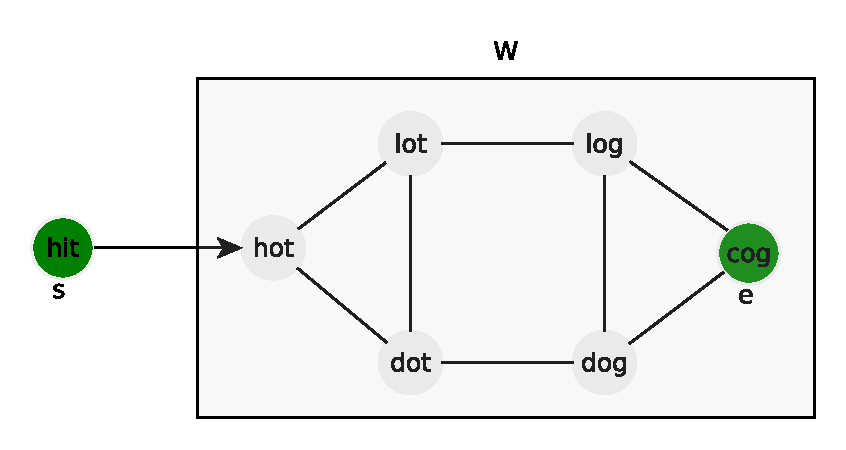
\includegraphics[width=\textwidth]{sources/word_ladder/images/example1}
        \caption[n]{Graph representation of Example \ref{example:word_ladder:example1}.}
        \label{fig:word_ladder:example1}
    \end{figure}
    \begin{figure}[]
        \centering
        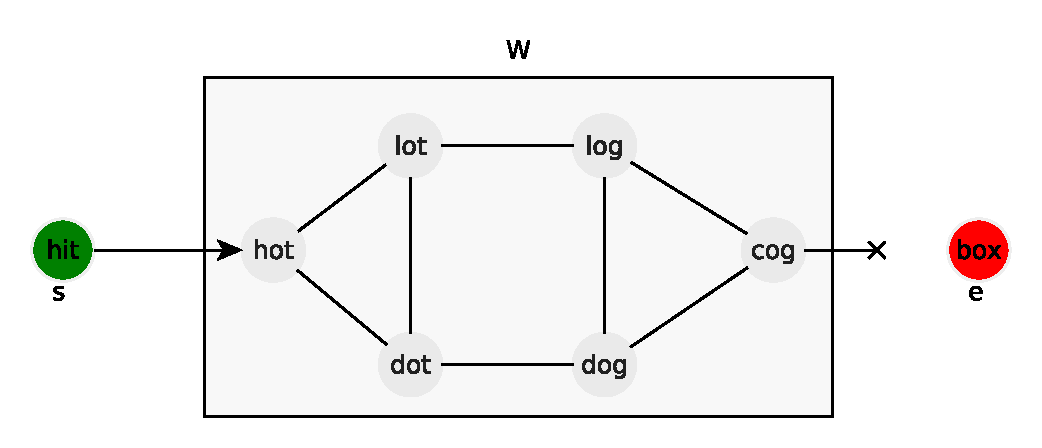
\includegraphics[width=\textwidth]{sources/word_ladder/images/example2}
        \caption[n]{Graph representation of Example \ref{example:word_ladder:example1} when $e=$\textit{box}. Notice how node \textit{box} is disconnected from the component containing \textit{hit}.}
        \label{fig:word_ladder:example1_impossible}
    \end{figure}
    

\lstinputlisting[language=c++, caption={Solution using BFS. Nodes different in exactly one character are connected.},label=list:word_ladder_bfs]{sources/word_ladder/word_ladder_solution1.cpp}

The code works by not explicitly constructing $G$ but instead by operating on an implicit graph. This implicit graph can be maintained by only keeping track of the visited nodes/words. 

\inline{word_ladder_BFS} is the main driver function and all it does is:
\begin{itemize}
    \item copying the elements of $W$ into an \inline{std::unordered_set} so that we can quickly check whether a string belongs to $W$ without having to perform a linear search.
    \item constructing a queue of \inline{std::pair<std:string, int>} as for each node/word we visit we want to remember its level (distance from $s$).
\end{itemize}.

The function \inline{addNeighbors} takes care of updating the BFS queue by generating all possible neighbors of a word $w$ having level \inline{count}. 
It does so by creating copies of $w$ that only differ in one position. If such a modified copy happens to be in $W$ then it is added to the queue with an incremented \inline{count} (signaling we need a step more to reach this new word from $w$).

The complexity of Listing \ref{list:word_ladder_bfs} is $O(|W|)$ for both time (albeit with a potentially high constant factor) and space.


%\chapter{Mini Problems}

\section{Greatest Common Divisor}
\begin{exercise}
    Write a function to calculate the GCD of two integers.
    \begin{example}
        \label{ex:gcd:example1}
        \hfill \\
        Given $35$ and $28$ the function returns $7$.
    \end{example}
    
    \begin{example}
        \label{ex:gcd:example2}
        \hfill \\
        Given $15$ and $8$ the function returns $1$.
    \end{example}

    \end{exercise}

\subsection{\CC Brute-force}
The GCD of two numbers $x$ and $y$ is defined as the largest integer that divides both $x$ and $y$. A simple and inefficient solution would simply loop over all numbers from the smallest between $x$ and $y$ and would stop as soon as we find one that divides both. We are guaranteed to find such a nuber as the number $1$ will happily divide any number. This solution is shown in Listing \ref{list:gcd_bruteforce}.

\lstinputlisting[language=c++, caption={Brute-force, linear time solution.},label=list:gcd_bruteforce]{test/mini_problems/gcd/gcd_bruteforce.cpp}

\subsection{Log-time solution. Euclidean Algorithm}
A much faster solution can be achieved by using the Euclidean algorithm for the GCD.
This algorithm is based on the principle that the greatest common divisor of two numbers $x$ and $y$ does not change if the larger number is replaced by the reminder of the integral division between $x$ and $y$.

For example, $21$ is the GCD of $252$ and $105$ (as $252 = 21 \times 12$ and $105 = 21 \times 5$), and the same number $21$ is also the GCD of $105$ and $252 \mod 105 = 42$.
Since this replacement reduces the larger of the two numbers, repeating this process gives successively smaller pairs of numbers until we reach a point where the smallest numbers divides the largest and therefore the reminder is zero (in the worst case the smallest becomes $1$). 

It was proven by Gabriel Lamé in 1844 that this algorithm always terminates in less steps than five times the number of digits of the smaller number (in base 10) making this algorithm extremely efficient as the number of digits grows logaritmically compared the number it represents.

Listing \ref{list:gcd_euclide} shows a recursive implementation of this algorithm while Listing \ref{list:gcd_euclide_iterative} shows an iterative one. 

\lstinputlisting[language=c++, caption={Euclide algorithm, recursive implementation.},label=list:gcd_euclide]{test/mini_problems/gcd/gcd_euclide.cpp}

\lstinputlisting[language=c++, caption={Euclide algorithm, iterative implementation.},label=list:gcd_euclide_iterative]{test/mini_problems/gcd/gcd_euclide_iterative.cpp}

\subsection{\CC Compile-time}
It is quite common to see specific requirements on the compile implementation of the GCD algorithm. Therefore in this section we will see how we can calculate the GCD in \CC at compile time. 

Before C++-11 the only way to do compile time computation was by using templates. In order to calculate GCD using templates we will use a structure with two integral template parameters that we will manipulate in a \inline{static const} variable. An implementation of this idea is shown in \ref{list:gcd_euclide_precpp11}.

\lstinputlisting[language=c++, caption={Pre C++11, compile-time template based solution.},label=list:gcd_euclide_precpp11]{test/mini_problems/gcd/gcd_euclide_pre_cpp11.cpp}

The code works by have a template class with two integral template parameters and a partial specialization that is used to terminate the recursion which is triggered whenever we request the static field \inline{::gcd}.

C++-11 introduces \inline{constexpr} function that can be used to specify function that can be run at compile-time. In C++-11 there are quite some limitation in what statements and operations we can do in a \inline{constexpr} context: for instance we can only have one return statement. Most of these contraints are related in the subsequent versions of the standard. A \inline{constexpr} recursive solution that works in C++-11 is shown in Listing \ref{list:gcd_euclide_cpp11}.

\lstinputlisting[language=c++, caption={C++11 \inline{constexpr} based solution.},label=list:gcd_euclide_cpp11]{test/mini_problems/gcd/gcd_euclide_cpp11.cpp}

Notice that, from C++-14 we can decorate Listing \ref{list:gcd_euclide_iterative} with \inline{constexpr} so that it can be used in compile-time computation.



%%%%%%%%%%%%%%%%%%%%%%%%%%%%%%%%%%%%%%%%%%%%%%%%%%%%%%%%%%%

\section{Maximum Depth of N-ary Tree}
\begin{exercise}
   Given a N-ary tree, return its depth which is defined as the length of the longest path from the tree's root to any of its leaves.
    \begin{example}
        \label{ex:nary-treedepth:example1}
        \hfill \\
        Given the tree depicted in Figure \ref{fig:longest_consecutive_sequence:example1} the function returns $3$ (path from node $1$ to node $12$).
    \end{example}
    
    \begin{example}
        \label{ex:nary-treedepth:example2}
        \hfill \\
        Given the tree depicted in Figure \ref{fig:longest_consecutive_sequence:example2} the function returns $6$ (path from node $1$ to node $40$).
    \end{example}
    \end{exercise}
 
 
\begin{figure}
	\centering
	\begin{subfigure}[]{0.45\textwidth}
		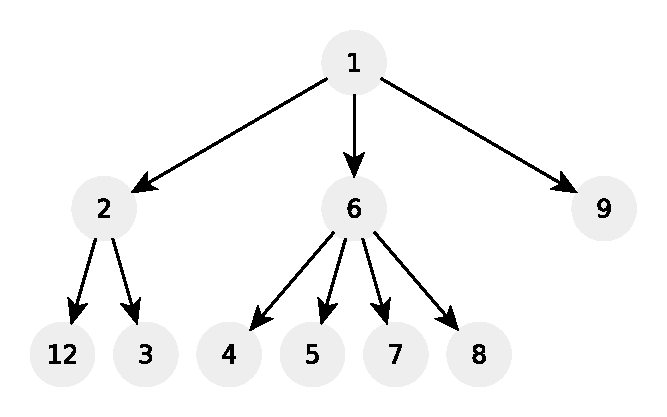
\includegraphics[width=1\linewidth]{sources/mini_problems/n-ary-tree-depth/images/example1}
		\caption{Input tree for Example \ref{ex:nary-treedepth:example1}.}
		\label{fig:longest_consecutive_sequence:example1}
	 \end{subfigure}
	\hfill
	\begin{subfigure}[]{0.45\textwidth}
		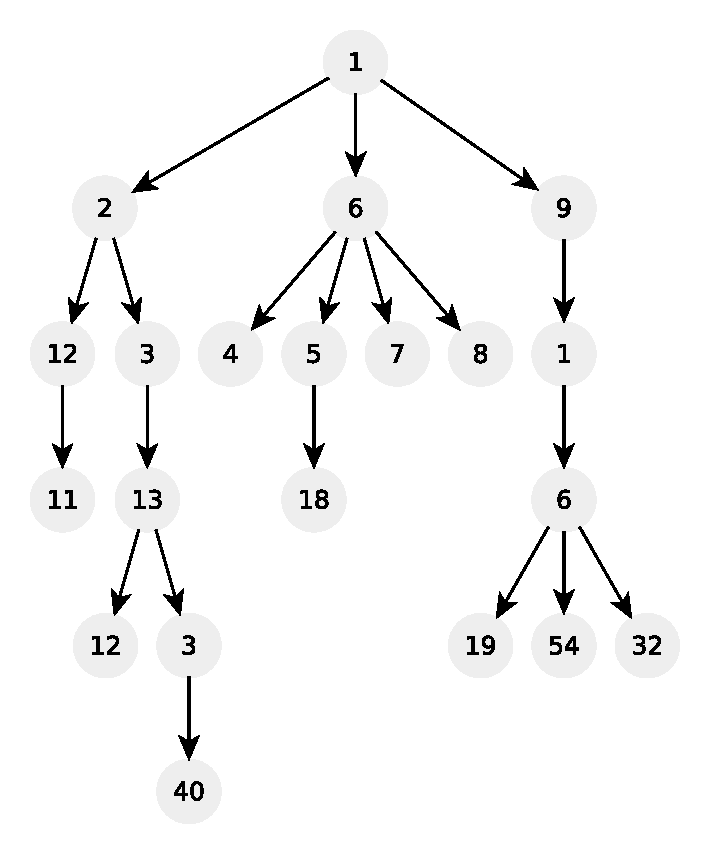
\includegraphics[width=1\linewidth]{sources/mini_problems/n-ary-tree-depth/images/example2}
		\caption{Input tree for Example \ref{ex:nary-treedepth:example2}.}
		\label{fig:longest_consecutive_sequence:example1}
	 \end{subfigure}
	 \caption[]{}
	  \label{}
\end{figure}
    
\subsection{Discussion}
    This is a classical problem, mostly asked during phone screening due to its simplicity. 
    What the problem, in other words, is asking us to do, is to return the maximum level of any of the tree's nodes.
    The level of a node is the number of its ancestors plus one. 
    Therefore to solve this problem, all we have to do is to visit the tree and keep track of the number of ancestors which is equivalent to the number of steps down the tree we took.
    We know that the root has $0$ ancestors and therefore, we know that each of its children will have $1$ ancestor (the root itself) and that any of its grandchildren will have $2$ ancestors and so on.
    
    Visiting a tree can be equally easily done recursively and iteratively as shown in Sections \ref{} and \ref{}, respectively.
 
    For the reminder of the discussion, we will define the root of a tree to be a pointer to the \inline{Node} structure defined in Listing \ref{list:n-arytreedepth:nodedef}.
 
    \begin{lstlisting}[language=c++, caption={Node definition.},label=list:n-arytreedepth:nodedef]]{
class Node {
public:
    int val;
    vector<Node*> children;

    Node() {}

    Node(int _val) {
        val = _val;
    }

    Node(int _val, vector<Node*> _children) {
        val = _val;
        children = _children;
    }
};            
    \end{lstlisting} 
    

\subsection{Recursive solution}
The recursive solution has the advantage of being shorter in terms of lines of code and in our opinion more elegant. It could, however, underperform the iterative solution if the compiler is not able to optimize the code properly or lead to out of memory errors if the tree depth goes over a certain value because at any given time, we keep in the stack a number of activation records that is equal to the level of the node we are visiting.

Listing \ref{list:n-ary-treedepth_recursive}  shows an implementation of this approach and has a linear time and space (considering the space occupied by the activation records) in the number of nodes of the tree.

\lstinputlisting[language=c++, caption={Recursive solution.},label=list:n-ary-treedepth_recursive]{test/mini_problems/n-ary-treedepth/n-ary-treedepth_recursive.cpp}

\subsection{Iterative Solution}
The same idea can be implemented iteratively as shown in Listing \ref{list:n-ary-treedepth_iterative} where we use a stack to keep track of the nodes \textbf{and their level}. Whenever we visit a node, we compare its level with the maximum found so far, then we remove it from the stack and insert all of its children in the stack with a level value increased by one. 

\lstinputlisting[language=c++, caption={Iterative solution.},label=list:n-ary-treedepth_iterative]{test/mini_problems/n-ary-treedepth/n-ary-treedepth_iterative.cpp}


%%%%%%%%%%%%%%%%%%%%%%%%%%%%%%%%%%%%%%%%%%%%%%%%%%%%%%%%%%%

\section{Assigning cookies \faCookie}
\begin{exercise}
    You are the parent of $n$ children and you want to make them happy by giving them a cookies (real ones  \faCookieBite, not HTTP cookie). 
    However you know that too many cookied are not good for them and therefore you settle for a rule that each child can at most get one cookie.
    Giving cookies to your children is not easy as they are special and each child $i$ has an integer greed factor $g[i]$ associated,
    which is the minimum size of a cookie that the child $i$ will be content with; 
    You have at your disposal a number $m$ of cookies, and each cookie $j$ has an integer size $s[j]$.
    You can give cookie number $i$ to child number $i$ if and only if $s[j] \ge g[i]$. When a child has a cookie assigned is content.
    
    Write a function that given a list  ($G$) of $n$ greed values and a list ($C$) of  $m$ cookie sizes determines the maximum possible of children you can make content.
     
    \begin{example}
        \label{ex:nary-treedepth:example1}
        \hfill \\
        Given $G=\{1,2,3\}$ and  $=\{1,1\}$ the function returns $1$. Despite having two cookies we can only make one child happy because we do not have cookies big enough for children number $2$ and $3$.
    \end{example}
    
    \begin{example}
        \label{ex:nary-treedepth:example2}
        \hfill \\
        Given $G=\{1,3\}$ and  $=\{1,4\}$ the function returns $2$. We can give the first cookie to the first child and the second cookie to the second child.
    \end{example}


    \begin{example}
        \label{ex:nary-treedepth:example3}
        \hfill \\
        Given $G=\{1,2,3\}$ and  $=\{1,1,3\}$ the function returns $2$. We can give the first cookie to the first child and the the third cookie to the second child The second cookie remains unassigned and the third child without cookie assigned.
    \end{example}
    \end{exercise}
 

\subsection{Discussion}
Let's start by noticing that despite what shown in the Exmaples the input lists are not guaranteed to be sorted and that, sorting actually makes solving this problem much easier.
The idea is that we have to find a way to assign to each children the smallest cookie possible that has size higher or equal to his greed. If the input array is not sorted then for each greed value we are forced to search $S$ entirely for a suitable cookie. 
If on the other hand both $G$ and $S$ are sorted then, we can try to accomodate children by increasing greed and keep track and assign progressively larger cookies to them. 
If a children with greed $i$ can be assigned cookie number $j$, then we can try to assign to child number $i+1$ cookie number $j+1$. If that does not work then we can try with cookie number $j+2$ and so on.
When we cannot assign a cookie $j$ to a certain child $i$, cookie $j$ will be unused, but that is not an issue because there is no way we can assign cookie $j$ to any other children because the greed values for children $i+1, i+2, \ldots$  will all be greater than the gree of child $i$.

Therefore in order to solve this problem we can:
\begin{itemize}
    \item sort $G$;
    \item sort $S$;
    \item use two pointers to keep track of the current child and current cookie
    \item process one child a the time until we ran out of children or cookies
    \item if the current cookie size is greater than the current child greed then we can advance both pointers
    \item otherwise we can only hope the next cookie will be assignable and therefore only advance the cookie pointer.
\end{itemize}

An implementation of this idea is shown in Listing \ref{list:assign_cookies_sorting}. Its time complexity is $O(nlog(n))$ while its the space complexity is $O(1)$.


\lstinputlisting[language=c++, caption={Solution using sorting.},label=list:assign_cookies_sorting]{test/mini_problems/assign_cookies/assign_cookies_sorting.cpp}


%%%%%%%%%%%%%%%%%%%%%%%%%%%%%%%%%%%%%%%%%%%%%%%%%%%%%%%%%%%

\section{Maximize Sum Of Array After K Negations}
\begin{exercise}
    Given an integer array $nums$ and an integer $k$, modify the array in the following way: choose an index $i$ and replace $nums[i]$ with $-nums[i]$.
    
    You should apply this process \textbf{exactly} $k$ times. You may choose the same index $i$ multiple times.
    
    Return the largest possible sum of all the elements of $nums$ at end of this process.     
    \begin{example}
        \label{ex:nary-treedepth:example1}
        \hfill \\
        Given $nums=\{4,2,3\}$ and $k=1$ the function returns $5$. We can choose index $1$ and turn the $2$ into $-2$. At the end we will be left with $nums=\{4,-2,3\}$ which totals to $4-2+3=5$.
    \end{example}
    
    \begin{example}
        \label{ex:nary-treedepth:example2}
        \hfill \\
        Given $nums=\{3,-1,0,2\}$ and $k=3$ the function returns $6$. We can choose 
    \end{example}


    \end{exercise}
 

\subsection{Discussion}
One easy way of solving this problem relies on the fact that all we have to do is to apply the change sign change always on the smallest number of the array.
The intuition behind it is that we should aim at first changing the sign of all the negative numbers first and among them we should prioritize the smallest ones: the number with the largest absolute value and negative sign. Changing the sign of those number will bring the best increase in the overall sum of the array.

If after having changed all negatives into positive we are left with more moved to make then we still have to change the sign of the smallest number in the array as many times as necessary.
This causes the smallest number of the array to switch sign back and forth until $k=0$ (this step can be optimized by noticing that if the number of moves left is even then the final valud of the smallest number in the array is not going to change, otherwise, it will be negative.We can reach this conclusion without having to actually perform the sign switch). 

To always keep track of the smallest number we can use a \inline{std::priority_queue} as shown in Listing \ref{}.

\lstinputlisting[language=c++, caption={Solution using sorting.},label=list:assign_cookies_sorting]{test/mini_problems/max_sum_array_after_k_negations/max_sum_array_after_k_negotiation_priority_queue.cpp}

The code works by applying the $k$ modifications always to the smallest element of the queue. At the end of the process we simply sum every element in the queue to obtain the answer. The complexity of this approach is $O(klog(n) + nlog(n))$ in time and $O(1)$ in space.


%%%%%%%%%%%%%%%%%%%%%%%%%%%%%%%%%%%%%%%%%%%%%%%%%%%%%%%%%%%

\section{Pairs of Songs With Total Durations Divisible by $k$}
\begin{exercise}
    You are given a list $T$ of songs where the $i^{th}$ song has a duration of $time[i]$ seconds.
    Write a function that given $T$ returns the number of distinct unordered pairs of songs for which the sum of their durations is divisible by an integer $k$.
    
    In other words,  the function should count the number of indices of $i < j$ such that $(T[i] + T[j]) \mod 60 == 0$.

     
    \begin{example}
        \label{ex:song_total_duration:example1}
        \hfill \\
        Given $T=\{30,20,150,100,40\}$ and $k=60$, the function returns $3$.
        We can pair songs at indices:
        \begin{itemize}
            \item $0$ and $2$ for a total duration of $180$;
             \item $1$ and $3$ for a total duration of $120$;
             \item $1$ and $4$ for a total duration of $60$.
        \end{itemize}
    \end{example}
    
    \end{exercise}
 

\subsection{Discussion}
This problem is quite similar to the two number sum problem discussed in Chapter \ref{ch:two_numbers_sum} and we will therefore use the very same technique to solve it (we will avoid discussing sub=optimal solution as the these are discussed already in the two number sum problem).
The difference here is that we are only interested in the number modulo $k$ and out main goal is to find two numbers whose remainder sum up to $0$.
For instance w.r.t. Example \ref{ex:song_total_duration:example1} we can see that  $T[0]+T[2] = 180$ which is divisible by $60$. 
If we have a look at their modulos are we notice that: $(T[0] \mod{60}) +(T[2] \mod{60}) = 30+30 = 60 \mod{60} =0$.
The same holds for the other two pairs of this example:
\begin{itemize}
    \item $(T[1] \mod{60}) +(T[3] \mod{60}) = 20+40 = 60 \mod{60} =0$
    \item $(T[1] \mod{60}) +(T[4] \mod{60}) = 20+40 = 60 \mod{60} =0$
\end{itemize}


Listing \ref{list:song_total_duration:lineartimespace} shows an implementation of this idea.

\lstinputlisting[language=c++, caption={Solution based on the two number sum problem.},label=list:song_total_duration:lineartimespace]{test/mini_problems/song_total_duration/song_total_duration_linear_time_space.cpp}



%%%%%%%%%%%%%%%%%%%%%%%%%%%%%%%%%%%%%%%%%%%%
%               Appendices
%%%%%%%%%%%%%%%%%%%%%%%%%%%%%%%%%%%%%%%%%%%%

\chapter{Appendices}
%% @Author: Davide Spataro
% @Date:   2020-10-25 
% @Last Modified by:   Davide Spataro
% https://www.topcoder.com/community/competitive-programming/tutorials/dynamic-programming-from-novice-to-advanced/
% file:///home/knotman/Downloads/DYNAMIC_PROGRAMMING_-_ITS_PRINCIPLES_APPLICATIONS_.pdf
% http://smo.sogang.ac.kr/doc/bellman.pdf 
\section*{Dynamic Programming}
\label{sect:appendix:DP}

Dynamic programming (DP) is a popular technique for solving a certain class of
optimization problems efficiently and is accredited to the American Scientist
Richard Bellman\cite{bellman1954}. He conied the term DP in the context of
solving problems involving a serie of best decision one after the other. 
The word \textit{programming} can be a bit deceiving for
computer scientist of programmers in general but it has really little to do with
computer programming and it is infact intended as a set of rules to 
follow to solve a certain problem and it is refeered specifically to the
solution to find an optimal military schedule for logistics (and has more or
less the same meaning as linear programming or linear optimization).  These rules can of course be coded and
executed by a computer but can be easily followed on paper for instance. 
Dynamic programming is better thought as an optimization approach rather than an
method or framework where a complex optimization problem is transformed into a sequence of
smaller (and simpler) problems. The very essence of DP is its multi-stage
optimization procedure. DP does not provide directly with the
instruction on how to solve a particular problem, but instead provides a general
framework that requires creativity and non trivial effort/insights so that a
problem formulation can be adapted and casted within the DP framework bounds.
This is possibly the reason why DP is considered a rather hard topic and it is
particularly feared during interviews. 

This chapter is not intended to be a full treatement of DP, and we will
introduce and describe it to the level that is necessary to understand and
better tackle DP interview problems. For a more comprenshive material on DP
please refer to \cite{bellman1954, cormen2009}.

The gist of the DP approach is that we aim at breaking down a problem into
simpler sub-problems recursively. If it is possible to do so, then the problem
at hand is said to have the \textbf{optimal substructure} property i.e. it can
be solved by using optimal solution to subproblems. But having the optimal
substructure property alone is not enough to prefer a DP approach to another
when trying to solve the same problem. This is because DP really shines when a
problem also exposes the \textbf{overlapping subproblems} property i.e. when the
subproblems are reused several times. A classic example if the
Fibonacci Sequence. In order to calculate $F(n)$ we need to solve two subproblems:
$F(n-1)$ and $F(n-2)$ and adding them up. But for solving $F(n-1)$ we need to
solve $F(n-2)$ \textbf{again}. The value for the subproblem $F(n-2)$ is thus
reused and this makes the Fibonacci problem exposed the optimal substructure
property. 
Dynamic programming takes care of this fact by making sure of solving each
subproblem only once. Usually this can be achieved into two ways:
\begin{description}
    \item [Top-down] This is usually the easiest of the two, by being a direct
    derivation from the recursive formulation of the problem. If the problem can
    be formulated recursively in terms of solution then solution to subproblems
    can be \textit{memoized}\footnote{From the latin word \textit{memorandum}
    which means to be remembered. It is basically a way of remembering the
    result of a function for a certain set of inputs call by storing it in a
    cache.} in a cache. 
    When a subproblem is reused then the
    (potentially expensive) recursive call is avoided and the cached result is
    returned instead. 
    \item [Bottom-up] We can try to reformulate the problem by twisting and
    massaging  the  recursive formulation so that the subproblems are solved
    first (thus effectively removing the recursion) and build the solution to
    the bigger problem from the bottom. This is usually done by working in a
    sort of tabular form where entries of the table for larger problems are
    filled by using  entries for solution to smaller problems that we have
    already solved. For instance, when solving the problem of finding the
    $10^{th}$ Fibonacci number $F(10)$, we can start from the known values for
    $F(0)$ and $F(1)$ and working our way up to $F(2)$  by using $F(1)$ and
    $F(2)$. Once F(2) is ready we can move up to F(3), and so on when we have
    the values for $F(8)$ and $F(9)$ we proceed with calculating $F(10)$.
\end{description}

DP has found application in many field of science such as Control theory,
Bioinformatics AI and operations research. There are a number of problems in
computer science that can be solved by using DP such as the 
\begin{itemize}
    \item Longest Common (or increasing) Subsequence
    \item Weighted Interval Scheduling
    \item Chain Matrix Multiplication
    \item Subset sub
    \item String edit distance
    \item Coin change
    \item 0/1 knapsack problem
    \item Graph shortest path
\end{itemize}

In the next section we will shortly review a number of DP problem focusing on
the key ideas that allow a problem to be approached and solved  using DP.

\subsection*{Fibonacci Sequence}
Computing the $n^{th}$ number of the Fibonacci sequence is probably one of the
most common introductionary example of DP. The Fibonacci sequence recursive
formulation is ready to be solved using a top-down DP approach. Listing
\ref{list:app:dp:canonical} shows a C++ function that calculated the $n^{th}$ Fibonacci
number.
\lstinputlisting[language=c++, caption={Canonical recursive C++ implementation of a function returning the $n^{th}$ Fibonacci number.},label=list:app:dp:canonical]{/home/dspataro/git/algorithm_articles/sources/appendices/fibonacci_canonical.cpp}
Notice that for instance when $F(6)$ a call tree is produced where the same call
is repeated more than once as shown in the list below. $F(2)$ has been
calculated $5$ times!
\begin{itemize}
    \item $F(6) = F(5)+F(4)$
    \item $F(6) = (F(4)+F(3)) + (F(3)+F(2))$
    \item $F(6) = ((F(3)+F(2))+(F(2)+F(1))) + ((F(2)+F(1))+(F(1)+F(0)))$
    \item $F(6) = (((F(2)+F(1))+(F(1)+F(0)))+((F(1)+F(0))+F(1))) + (((F(1)+F(0))+F(1))+(F(1)+F(0)))$
    \item $F(6) = ((((F(1)+F(0))+F(1))+(F(1)+F(0)))+((F(1)+F(0))+F(1))) + (((F(1)+F(0))+F(1))+(F(1)+F(0)))$
\end{itemize}

Listing \ref{list:app:dp:fib} can be improved dramatically if we memoize the function calls
that have been already calculated. This way no duplicate work is done. W.r.t the
previous example, from the second time the value of $F(2)$ is needed, no
additional work is done, as the value in the cache is returned.
\lstinputlisting[language=c++, caption={Canonical recursive top-down Dynamic Programming C++ implementation of a function returning the $n^{th}$ Fibonacci number.},label=list:app:dp:fib]{/home/dspataro/git/algorithm_articles/sources/appendices/fibonacci_dp_top_down.cpp}

%\section{Prefix sum}
\label{sect:appendix:prefix_sum}
In computer science, the prefix sum, cumulative sum, inclusive scan, or simply scan of a sequence of numbers x0, x1, x2, ... is a second sequence of numbers y0, y1, y2, ..., the sums of prefixes (running totals) of the input sequence:
%% @Author: Davide Spataro
% @Date:   2020-03-30 17:18:14
% @Last Modified by:   Davide Spataro
% @Last Modified time: 2020-03-30 17:28:08
\section{Binary Search}
\label{sect:appendix:binary_search}
\lipsum{1}
\lstinputlisting[language=c++, caption={},label=list:listings:hash_pair]{test/common/hash_pair.h}

\section*{Latencies Reference}
\FloatBarrier
\begin{table}[]
    \centering
    \resizebox{\textwidth}{!}{%
    \begin{tabular}{lllll}
    \hline
    \rowcolor[HTML]{C0C0C0} 
    \multicolumn{1}{c}{\cellcolor[HTML]{C0C0C0}\textbf{Operation}}     & \multicolumn{3}{c}{\cellcolor[HTML]{C0C0C0}\textbf{Latency}}               & \multicolumn{1}{c}{\cellcolor[HTML]{C0C0C0}\textbf{Notes}} \\ \hline
    \rowcolor[HTML]{C0C0C0} 
                                                                       & \textit{\textbf{nano}} & \textit{\textbf{micro}} & \textit{\textbf{milli}} &                                                            \\
    \textit{L1 cache reference}                                        & 0.5                    & 0.000500000             & 0.000000500             & 14 \textbackslash{}times L1 cache                          \\
    \textit{Branch mispredict}                                         & 5                      & 0.005000000             & 0.000005000             &                                                            \\
    \textit{L2 cache reference}                                        & 7                      & 0.007000000             & 0.000007000             &                                                            \\
    \textit{Mutex lock/unlock}                                         & 25                     & 0.025000000             & 0.000025000             &                                                            \\
    \textit{Main Memory Reference}                                     & 100                    & 0.100000000             & 0.000100000             & 20 times L2 cache. 200x L1                                 \\
    \textit{Compress 1K bytes with Zippy}                              & 3000                   & 3.000000000             & 0.003000000             &                                                            \\
    \textit{Send 1K bytes over 1 Gbps network}                         & 10000                  & 10.000000000            & 0.010000000             &                                                            \\
    \textit{Read 4K randomly from SSD*}                                & 150000                 & 150.000000000           & 0.150000000             & $\sim$1GB/sec SSD                                          \\
    \textit{Round trip within same datacenter}                         & 500000                 & 500.000000000           & 0.500000000             &                                                            \\
    \textit{Read 1 MB sequentially from SSD*}                          & 1000000                & 1000.000000000          & 1.000000000             & $\sim$1GB/sec SSD, 4X memory                               \\
    \textit{Disk seek}                                                 & 10000000               & 10000.000000000         & 10.000000000            & 20x datacenter roundtrip                                   \\
    \textit{Read 1 MB sequentially from disk}                          & 20000000               & 20000.000000000         & 20.000000000            & 80x memory, 20X SSD                                        \\
    \textit{Send packet CA-\textgreater{}Netherlands-\textgreater{}CA} & 150000000              & 150000.000000000        & 150.000000000           &                                                           
    \end{tabular}%
    }
    \caption{Latency Comparison Numbers ($\sim$2012). Credit to \url{https://gist.github.com/jboner/2841832}}
    \label{tab:refernce_latencies}
\end{table}
\FloatBarrier


\begin{figure}
	\centering
	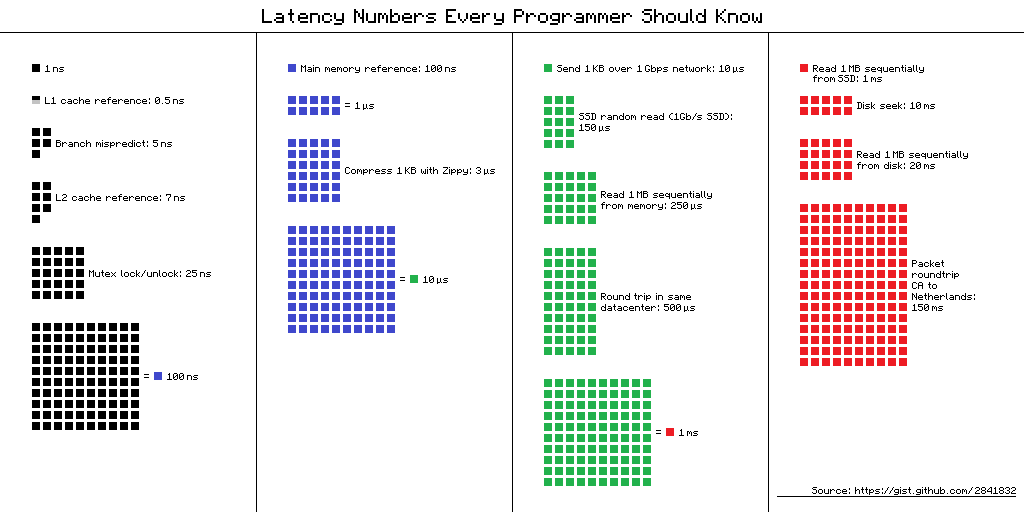
\includegraphics[width=\textwidth]{sources/appendices/images/latencies-refernece.png}
	\caption[]{Humanized visualization of the data in Table 
    \ref{tab:refernce_latencies}}.
	\label{fig:refernce_latencies}
\end{figure}

\FloatBarrier

\vspace{-2cm}
\section*{Data structures Asymptotic complexity cheatsheet}
% Please add the following required packages to your document preamble:
% \usepackage{booktabs}
% \usepackage{multirow}
% \usepackage{graphicx}
% \usepackage[table,xcdraw]{xcolor}
% If you use beamer only pass "xcolor=table" option, i.e. \documentclass[xcolor=table]{beamer}
\begin{table}[!htbp]
    \centering
    \resizebox{\textwidth}{!}{%
    \begin{tabular}{@{}lccccccccc@{}}
    \toprule
                                              & \multicolumn{8}{l}{\textbf{Time Complexities}}                                                                                                                                                                                                                                                                                                                                                  & \multicolumn{1}{l}{\textbf{Space Complexity}}             \\ \cmidrule(l){2-10} 
                                              & \multicolumn{1}{l}{\textbf{Average case}}    & \multicolumn{7}{l}{\textbf{Worst case}}                                                                                                                                                                                                                                                                                                          & \multicolumn{1}{l}{}                                      \\
    \multirow{-3}{*}{\textbf{Data Structure}} & \multicolumn{1}{l}{\textit{\textbf{Access}}} & \multicolumn{1}{l}{\textit{\textbf{Search}}} & \multicolumn{1}{l}{\textit{\textbf{Insertion}}} & \multicolumn{1}{l}{\textit{\textbf{Deletion}}} & \multicolumn{1}{l}{\textit{\textbf{Access}}} & \multicolumn{1}{l}{\textit{\textbf{Search}}} & \multicolumn{1}{l}{\textit{\textbf{Insertion}}} & \multicolumn{1}{l}{\textit{\textbf{Deletion}}} & \multicolumn{1}{l}{\multirow{-2}{*}{\textbf{Worst case}}} \\ \cmidrule(r){1-1}
    Array                                     & \cellcolor[HTML]{009901}$O(1)$               & \cellcolor[HTML]{FFC702}$O(n)$               & \cellcolor[HTML]{FFC702}$O(n)$                  & \cellcolor[HTML]{FFC702}$O(n)$                 & \cellcolor[HTML]{009901}$O(1)$               & \cellcolor[HTML]{FFC702}$O(n)$               & \cellcolor[HTML]{FFC702}$O(n)$                  & \cellcolor[HTML]{FFC702}$O(n)$                 & \cellcolor[HTML]{FFC702}$O(n)$                            \\
    Stack                                     & \cellcolor[HTML]{009901}$O(1)$               & \cellcolor[HTML]{656565}N.A.                 & \cellcolor[HTML]{009901}$O(1)$                  & \cellcolor[HTML]{009901}$O(1)$                 & \cellcolor[HTML]{009901}$O(1)$               & \cellcolor[HTML]{656565}N.A.                 & \cellcolor[HTML]{009901}$O(1)$                  & \cellcolor[HTML]{009901}$O(1)$                 & \cellcolor[HTML]{FFC702}$O(n)$                            \\
    Queue                                     & \cellcolor[HTML]{009901}$O(1)$               & \cellcolor[HTML]{656565}N.A.                 & \cellcolor[HTML]{009901}$O(1)$                  & \cellcolor[HTML]{009901}$O(1)$                 & \cellcolor[HTML]{009901}$O(1)$               & \cellcolor[HTML]{656565}N.A.                 & \cellcolor[HTML]{009901}$O(1)$                  & \cellcolor[HTML]{009901}$O(1)$                 & \cellcolor[HTML]{FFC702}$O(n)$                            \\
    Singly Linked List                        & \cellcolor[HTML]{FFC702}$O(n)$               & \cellcolor[HTML]{FFC702}$O(n)$               & \cellcolor[HTML]{009901}$O(1)$                  & \cellcolor[HTML]{FFC702}$O(n)$                 & \cellcolor[HTML]{FFC702}$O(n)$               & \cellcolor[HTML]{FFC702}$O(n)$               & \cellcolor[HTML]{009901}$O(1)$                  & \cellcolor[HTML]{FFC702}$O(n)$                 & \cellcolor[HTML]{FFC702}$O(n)$                            \\
    Doubly Linked List                        & \cellcolor[HTML]{FFC702}$O(n)$               & \cellcolor[HTML]{FFC702}$O(n)$               & \cellcolor[HTML]{009901}$O(1)$                  & \cellcolor[HTML]{009901}$O(1)$                 & \cellcolor[HTML]{FFC702}$O(n)$               & \cellcolor[HTML]{FFC702}$O(n)$               & \cellcolor[HTML]{009901}$O(1)$                  & \cellcolor[HTML]{009901}$O(1)$                 & \cellcolor[HTML]{FFC702}$O(n)$                            \\
    Hash Table                                & \cellcolor[HTML]{009901}$O(1)$               & \cellcolor[HTML]{009901}$O(1)$               & \cellcolor[HTML]{009901}$O(1)$                  & \cellcolor[HTML]{009901}$O(1)$                 & \cellcolor[HTML]{FFC702}$O(n)$               & \cellcolor[HTML]{FFC702}$O(n)$               & \cellcolor[HTML]{FFC702}$O(n)$                  & \cellcolor[HTML]{FFC702}$O(n)$                 & \cellcolor[HTML]{FFC702}$O(n)$                            \\
    Binary Search Tree                        & \cellcolor[HTML]{32CB00}$O(log_2(n))$        & \cellcolor[HTML]{32CB00}$O(log_2(n))$        & \cellcolor[HTML]{32CB00}$O(log_2(n))$           & \cellcolor[HTML]{32CB00}$O(log_2(n))$          & \cellcolor[HTML]{FFC702}$O(n)$               & \cellcolor[HTML]{FFC702}$O(n)$               & \cellcolor[HTML]{FFC702}$O(n)$                  & \cellcolor[HTML]{FFC702}$O(n)$                 & \cellcolor[HTML]{FFC702}$O(n)$                            \\
    Red-Black Tree                            & \cellcolor[HTML]{32CB00}$O(log_2(n))$        & \cellcolor[HTML]{32CB00}$O(log_2(n))$        & \cellcolor[HTML]{32CB00}$O(log_2(n))$           & \cellcolor[HTML]{32CB00}$O(log_2(n))$          & \cellcolor[HTML]{32CB00}$O(log_2(n))$        & \cellcolor[HTML]{32CB00}$O(log_2(n))$        & \cellcolor[HTML]{32CB00}$O(log_2(n))$           & \cellcolor[HTML]{32CB00}$O(log_2(n))$          & \cellcolor[HTML]{FFC702}$O(n)$                            \\
    Heap                                      & \cellcolor[HTML]{009901}$O(1)$               & \cellcolor[HTML]{656565}N.A.                 & \cellcolor[HTML]{32CB00}$O(log_2(n))$           & \cellcolor[HTML]{32CB00}$O(log_2(n))$          & \cellcolor[HTML]{009901}$O(1)$               & \cellcolor[HTML]{656565}N.A.                 & \cellcolor[HTML]{32CB00}$O(log_2(n))$           & \cellcolor[HTML]{32CB00}$O(log_2(n))$          & \cellcolor[HTML]{FFC702}$O(n)$                            \\ \bottomrule
    \end{tabular}%
    }
    \caption{Asymptotic complexities for a number of data strucutes. For time, both the average and case is reported, while for space only the worst. $O(1) < O(log_2(n)) < O(log_2(n)) < O(n) < O(nlog_2(n) < O(n^2) < O(n^3) \ldots < O(2^n) < O(n!) < O(n^n)$  }
    \label{appendix:ds_complexities}
\end{table}


\begin{figure}
    \centering
\begin{tikzpicture}
    \begin{axis}[
      grid = major,
      clip = true,
      ticks = none,
      width=0.9\textwidth,
      height=0.7\textwidth,
      every axis plot/.append style={very thick},
      axis line style = ultra thick,
      clip mode=individual,
      restrict y to domain=0:40,
      restrict x to domain=0:20,
      axis x line = left,
      axis y line = left,
      domain = 0.00:10,
      xmin = 0,
      xmax = 11,
      ymin = 0,
      ymax = 42,
      xlabel = n,
      ylabel = no. of operations,
      xlabel style = {at={(axis description cs:0.5,-0.1)},anchor=south},
      ylabel style = {at={(axis description cs:-0.08,0.5)},anchor=north},
      label style = {font=\LARGE\bf},
    ]
  \addplot [
      samples=100, 
      color=red,
  ]
  {x^2}node[above,pos=1,style={font=\Large}]{$\mathcal{O}(n^2)$};
  \addplot [
      samples=100, 
      color=blue,
  ]
  {x}node[above,pos=1,style={font=\Large}]{$\mathcal{O}(n)$};
  \addplot [
      samples=100, 
      color=orange,
  ]
  {log2 x}node[above,pos=1,style={font=\Large}]{$\mathcal{O}(\log{}n)$};
  \addplot [
      samples=100, 
      color=black,
  ]
  {x*(log2 x)}node[above,pos=1,style={font=\Large}]{$\mathcal{O}(n\log{}n)$};
  \addplot [
      samples=100, 
      color=magenta,
  ]
  {1}node[above,pos=1,style={font=\Large}]{$\mathcal{O}(1)$};
  \addplot [
      samples=100, 
      color=cyan,
  ]
  {x^(2.2)}node[above,pos=1,style={font=\Large}]{$\mathcal{O}(n^3)$};
  

  \addplot [
    samples=100,
    color=green, 
  ] gnuplot{gamma(x+3)} node[above,pos=1,style={font=\Large}]{$\mathcal{O}(n!)$};

  \addplot [
    samples=100, 
    color=yellow,
]
{2.5*2^x}node[above,pos=1,style={font=\Large}]{$\mathcal{O}(2^x)$};
  
  \end{axis}
  \end{tikzpicture}

  \caption[]{Graph showing the relative growth rates of common function used to describe algorithms.}
  \label{fig:ds_complexities:graph}
\end{figure}
%%%%%%%%%%%%%%%%%%%%%%%%%%%%%%%%%%%%%%%%%%%%
%               BIBLIOGRAPHY
%%%%%%%%%%%%%%%%%%%%%%%%%%%%%%%%%%%%%%%%%%%%

%
%from documentation
%\newacronym[⟨key-val list⟩]{⟨label ⟩}{⟨abbrv ⟩}{⟨long⟩}
%above is short version of this
% \newglossaryentry{⟨label ⟩}{type=\acronymtype,
% name={⟨abbrv ⟩},
% description={⟨long⟩},
% text={⟨abbrv ⟩},
% first={⟨long⟩ (⟨abbrv ⟩)},
% plural={⟨abbrv ⟩\glspluralsuffix},
% firstplural={⟨long⟩\glspluralsuffix\space (⟨abbrv ⟩\glspluralsuffix)},
% ⟨key-val list⟩}

\newacronym{cd}{CD}{compact disk}
\newacronym{utc}{UTC}{Coordinated Universal Time}
%\newacronym{adt}{ADT}{Atlantic Daylight Time}
%\newacronym{est}{EST}{Eastern Standard Time}
 
% Use the acronyms
\gls{utc} is 3 hours behind \gls{adt} and 10 hours ahead of \gls{est}.



%\addcontentsline{toc}{chapter}{\textcolor{ocre}{Glossary}}
%\printglossaries


%Print the glossary

\addcontentsline{toc}{chapter}{\textcolor{ocre}{Bibliography}}
%\chapter*{Bibliography}
%Print the glossary
\printbibliography	
	
%%%%%%%%%%%%%%%%%%%%%%%%%%%%%%%%%%%%%%%%%%%%
%               INDEX
%%%%%%%%%%%%%%%%%%%%%%%%%%%%%%%%%%%%%%%%%%%%	
	\cleardoublepage
	\phantomsection
	\setlength{\columnsep}{0.75cm}
	\addcontentsline{toc}{chapter}{\textcolor{ocre}{Index}}
	\printindex


	%\backmatter

\end{document}
